\documentclass{standalone}
\usepackage{pgfplots}
\begin{document}

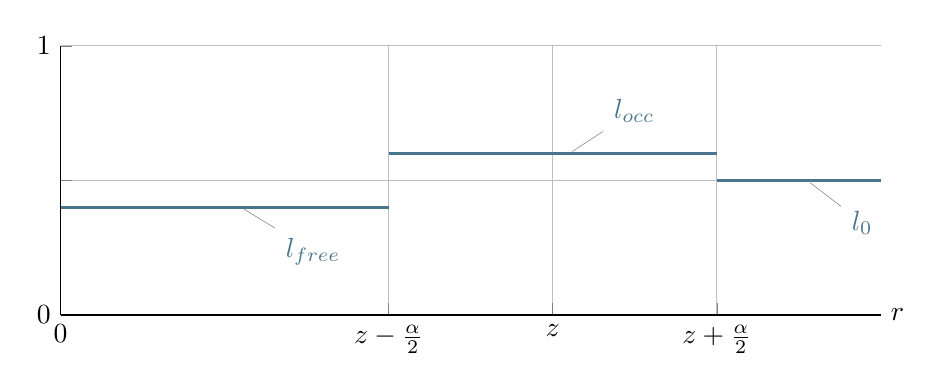
\begin{tikzpicture}
\begin{axis}[
  no markers, domain=0:10, samples=100,
  axis lines*=left, xlabel=$r$, %ylabel=$l_r$,
  every axis y label/.style={at=(current axis.above origin),anchor=south},
  every axis x label/.style={at=(current axis.right of origin),anchor=west},
  height=5cm, width=12cm,
  xtick={0,4,6,8}, xticklabels={0,$z - \frac{\alpha}{2}$,$z$,$z + \frac{\alpha}{2}$},
  ytick={0,0.5,1}, yticklabels={0,,1},
  enlargelimits=false, clip=false,
  grid = major
  ]
  \addplot [draw=none] {1};
  \addplot [draw=none] {0};

  \addplot [very thick,cyan!50!black, domain=0:4] {0.4} node [pos=0.55,pin={-30:$l_{free}$},inner sep=0pt] {};
  \addplot [very thick,cyan!50!black, domain=4:8] {0.6} node [pos=0.55,pin={30:$l_{occ}$},inner sep=0pt] {};
  \addplot [very thick,cyan!50!black, domain=8:10] {0.5} node [pos=0.55,pin={-30:$l_0$},inner sep=0pt] {};

%\draw [yshift=-0.6cm, latex-latex](axis cs:4,0) -- node [fill=white] {$1.96\sigma$} (axis cs:5.96,0);
\end{axis}


\end{tikzpicture}
\end{document}